\documentclass[pdflatex,sn-mathphys-num,iicol]{sn-jnl}

\usepackage[T1]{fontenc}
\usepackage{amsmath,amssymb}
\usepackage{algorithm}
\usepackage{algpseudocode}
\algrenewcommand\algorithmicrequire{\textbf{Input:}}
\algrenewcommand\algorithmicensure{\textbf{Output:}}
\usepackage{booktabs}
\usepackage{array}
\usepackage{graphicx}
\usepackage{tikz}
\usepackage{pgfplots}
\pgfplotsset{compat=1.17}
\usetikzlibrary{arrows.meta,calc,positioning,patterns}
\hypersetup{hypertexnames=false}
\renewcommand{\topfraction}{0.9}
\renewcommand{\bottomfraction}{0.8}
\renewcommand{\textfraction}{0.07}
\renewcommand{\floatpagefraction}{0.8}
\renewcommand{\dbltopfraction}{0.9}
\renewcommand{\dblfloatpagefraction}{0.6}
\setcounter{topnumber}{3}
\setcounter{bottomnumber}{2}
\setcounter{totalnumber}{5}
\setcounter{dbltopnumber}{3}
\setlength{\floatsep}{12pt plus 3pt minus 2pt}
\setlength{\textfloatsep}{12pt plus 3pt minus 2pt}
\setlength{\dblfloatsep}{12pt plus 3pt minus 2pt}
\setlength{\dbltextfloatsep}{12pt plus 3pt minus 2pt}
\newcommand{\ci}[3]{\begin{tabular}[c]{@{}c@{}}$#1$\\{}[$#2$, $#3$]\end{tabular}}
\newcommand{\cib}[3]{{\boldmath\ci{#1}{#2}{#3}}}
\newcommand{\cit}[3]{\begin{tabular}[t]{@{}c@{}}$#1$\\{}[$#2$, $#3$]\end{tabular}}
\newcommand{\cibt}[3]{{\boldmath\cit{#1}{#2}{#3}}}
\newcommand{\scl}{SCL}
\newcommand{\aob}{AOB}
\newcommand{\twol}[2]{\begin{tabular}[c]{@{}l@{}}#1\\#2\end{tabular}}

\makeatletter
\def\email#1{\global\advance\emailcnt by 1\relax
\if@corauemail
  \ifx\corrauthemail\@empty\g@addto@macro\corrauthemail{\textcolor{blue}{#1}}%
  \else\g@addto@macro\corrauthemail{;\ \textcolor{blue}{#1}}\fi
\else
  \ifx\authemail\@empty\g@addto@macro\authemail{\textcolor{blue}{#1}}%
  \else\g@addto@macro\authemail{;\ \textcolor{blue}{#1}}\fi
\fi}
\makeatother

\begin{document}

\title[Self-Calibrating Control Layer for Multi-Object Trackers]{Training-Free Self-Calibrating Control Layer for Heterogeneous Multi-Object Trackers}

\author*[1]{\fnm{Ahmed Gouda} \sur{Ismail}}\email{a7medgouda1@gmail.com}
\author[1]{\fnm{Mohamed S.} \sur{Mohamed}}\email{mohamedms@mtc.edu.eg}
\author[2]{\fnm{Tarek Ahmed} \sur{Mahmoud}}\email{tarek.mohamed@eui.edu.eg}

\affil*[1]{\orgdiv{Computer Engineering and Artificial Intelligence Department}, \orgname{Military Technical College}, \orgaddress{\city{Cairo}, \country{Egypt}}}
\affil[2]{\orgdiv{Computer Engineering Department}, \orgname{Egypt University of Informatics}, \orgaddress{\city{Cairo}, \country{Egypt}}}

\abstract{Multi-object tracking systems combine a detector, which finds objects and gives each a confidence score, with a tracker, which links them over time using fixed score thresholds. When the detector is replaced, retrained, or compressed, its scores change, but the tracker keeps its old thresholds. This paper proposes a training-free self-calibrating control layer (\scl{}) placed between an unchanged detector and tracker (the host). It splits the scores of recent frames with Otsu's histogram threshold and labels their distribution as clean or noisy. On clean scores it keeps the host's scores; on noisy scores it chooses which detections reach the host, rescores them, and sets its thresholds. It also continues tracks through low-score frames for single-stage trackers. It needs no labels or future frames. One fixed configuration was tested on seven published trackers, four detection sources, and three datasets. All gains below are relative changes over the tracker alone. \scl{} raises the higher order tracking accuracy (HOTA) of two single-stage trackers by 0.9\%: OC-SORT, used during development, and PD-SORT, which was not. With halved detector scores, two trackers failed; with \scl{}, both recovered at least 97\% of their original HOTA. With a noisy RT-DETR-L detector, \scl{} raises the multiple object tracking accuracy (MOTA) of ByteTrack and BoT-SORT by 12.6\% and 16.3\% and reduces their identity switches by 43\% and 47\%. On four trackers that already fit their detections, HOTA changed by less than 0.1\%. Paired bootstrap analysis supports these results. \scl{} adds 2.95 milliseconds per frame on an ordinary processor.}

\keywords{multi-object tracking, tracking by detection, detector confidence calibration, online adaptation, Otsu thresholding, real-time image processing}

\maketitle

\section{Introduction}\label{sec:intro}

Multi-object tracking (MOT) finds every object of interest in a video and gives each one an
identity number (ID) that stays the same over time. It is used in surveillance, driving, and drone
systems \cite{zhu2022visdrone,wu2022uavsurvey}, where results are needed with little delay. Most
MOT systems follow the tracking-by-detection design \cite{adzemovic2026survey}: in each frame, a
detector returns candidate boxes with confidence scores, and a tracker links them into tracks, one
per object \cite{bewley2016sort,zhang2022bytetrack,cao2023ocsort}. The tracker uses a box only if
its score passes a fixed threshold. A two-stage tracker, such as ByteTrack, also uses lower-score
boxes in a second step to continue unmatched tracks \cite{zhang2022bytetrack}; a single-stage
tracker, such as OC-SORT, ignores every box below one threshold \cite{cao2023ocsort}.

In real systems the detector is often replaced, retrained, or compressed, while the tracker keeps
the thresholds that its authors set for another detector. Detector scores are not calibrated across
models and conditions \cite{kuppers2020detcalib}, so a new detector usually gives scores on a
different scale, and nothing in the system notices. The effect can be large: halving the scores of
a published detector reduces two well-known trackers to 0 higher order tracking accuracy (HOTA)
\cite{luiten2021hota}, because no detection passes their thresholds (Sect.~\ref{sec:shift}).
Retuning every tracker for every detector needs labels, which a working system usually does not
have. Adaptive-threshold methods are each built into one tracker
\cite{ma2023adaptivebytetrack,shim2024adaptrack,act2026adaptive}, score calibration needs
labelled data \cite{kuppers2020detcalib}, and adaptive inference methods learn their settings for
one model \cite{han2022dynamic,jiang2018chameleon}.

This paper presents a self-calibrating control layer (\scl{}) that sits between a detector and a
tracker that are both kept fixed (frozen): their code, weights, and stored settings are not
changed. We call the tracker that \scl{} serves the \emph{host}; it gives \scl{} four of its
published settings, the host contract (Sect.~\ref{sec:contract}). \scl{} checks how many of the
higher scores of recent frames form a clearly confident group, using only the scores, so it needs
no labels. If most are confident, the host keeps its scores and, unless they would reject the
confident group, its thresholds, and the layer only adds a step that continues tracks. If many are uncertain, \scl{} chooses which candidates reach the host, gives
them new scores, and sets the host's thresholds for the frame.

With halved detector scores, \scl{} restored two trackers from 0 to about 66 HOTA; with other
detectors, it raised the multiple object tracking accuracy (MOTA) of two-stage trackers by up to
24.7 points and cut their identity switches by 43\% to 56\%, while well-matched strong trackers
stayed within 0.06 HOTA points of their own accuracy.

The main contributions are:
\begin{enumerate}
\item \scl{}, a training-free and causal layer that keeps the tracker's scores and thresholds when
      the scores are clean, lowering a threshold only if it would reject the confident group, and
      takes control only when they are noisy, with a host contract that lets one fixed
      configuration serve single-stage and two-stage trackers without changing them
      (Sect.~\ref{sec:method}).
\item A development path from always-on banding (\aob{}), an earlier design that always
      intervened, in which each step is compared with the step it was built on
      (Sect.~\ref{sec:development}).
\item An evaluation of one frozen configuration with paired bootstrap intervals, comparisons with
      simple adaptive thresholds and the published ACT method, an analysis of each part of the
      layer (Sect.~\ref{sec:results}), and a cost of about 3 ms per frame on an ordinary processor
      (central processing unit, CPU) (Sect.~\ref{sec:cost}).
\end{enumerate}

Section~\ref{sec:related} covers the data, metrics, and related work;
Sections~\ref{sec:method} and~\ref{sec:development} present \scl{} and its development;
Section~\ref{sec:results} gives the results; and Sections~\ref{sec:discussion}
and~\ref{sec:conclusion} discuss and conclude.

\section{Background and Related Work}\label{sec:related}

\subsection{Datasets}\label{sec:data}
Three public datasets are used. \emph{MOT17} \cite{milan2016mot16} contains 14 sequences of
people filmed with static and moving cameras. As is common, the second half of each of the seven
training sequences, called val-half (2,652 frames), is used for evaluation \cite{zhang2022bytetrack},
with the published YOLOX-X detections \cite{ge2021yolox} at the two published emission floors, the
lowest scores emitted, of 0.01 and 0.1. To study score changes directly, these scores were also
changed before the tracker by four transforms that keep their order: cubing ($s^3$), halving
($0.5\,s$), and logit temperatures $T=2$ and $T=0.5$, which divide the logit of each score by $T$.
\emph{KITTI tracking} \cite{geiger2012kitti} has 21 training sequences (8,008 frames) recorded from
a car and is scored on cars and pedestrians; here the trackers run with two other detectors,
YOLOv8n \cite{jocher2023yolov8} and RT-DETR-L \cite{zhao2024rtdetr}, and keep thresholds that were
set for other detectors. \emph{UAVDT} \cite{du2018uavdt} contains drone videos of vehicles; its 20
test sequences (16,592 frames) are used with ByteTrack, YOLOv8n, and RT-DETR-L.

MOT17 with four trackers, KITTI, and the score transforms were development data, looked at while
\scl{} was designed. Two predeclared external trackers, PD-SORT and Hybrid-SORT, were chosen in
advance and run once with the frozen configuration on the detections released by their authors on
MOT17 val-half. The held-out UAVDT test split was also run once, after a written plan. Each
external host was checked against its authors' number: EXACT within 0.2 HOTA points, CLOSE within
1.0.

\subsection{Evaluation metrics}\label{sec:metrics}
HOTA \cite{luiten2021hota}, the main metric, balances finding the objects and keeping their
identities,
\begin{equation}
\mathrm{HOTA}=\frac{1}{19}\sum_{\alpha}\sqrt{\mathrm{DetA}_\alpha\,\mathrm{AssA}_\alpha},
\label{eq:hota}
\end{equation}
where $\mathrm{DetA}_\alpha$ and $\mathrm{AssA}_\alpha$ are the detection and association accuracy
at the localization threshold $\alpha=0.05,0.10,\dots,0.95$. MOTA \cite{bernardin2008clear} and
IDF1 \cite{ristani2016idf1} are
\begin{align}
\mathrm{MOTA}&=1-\frac{\mathrm{FN}+\mathrm{FP}+\mathrm{IDS}}{\mathrm{GT}},\label{eq:mota}\\
\mathrm{IDF1}&=\frac{2\,\mathrm{IDTP}}{2\,\mathrm{IDTP}+\mathrm{IDFP}+\mathrm{IDFN}},\label{eq:idf1}
\end{align}
where FN are missed objects (false negatives), FP false positives, IDS identity switches (an
object's ID changes), and GT the number of ground-truth boxes; IDTP, IDFP, and IDFN count boxes
after each ground-truth track is matched to at most one output track. All metrics are computed
with TrackEval (commit 12c8791) and the official ground truth \cite{dendorfer2021motchallenge};
KITTI HOTA is averaged over cars and pedestrians, and on UAVDT all vehicles form one class and
predictions in ignored regions are removed. HOTA, MOTA, and IDF1 are in percent, and differences
in points.

All comparisons are paired: each tracker runs alone and with \scl{} on the same sequences and
detections. Paired bootstrap resampling of whole sequences \cite{efron1993bootstrap}, 10,000 times
with seed 42, gives a 95\% interval (2.5--97.5 percentiles) for each difference, which is called
significant when its interval does not include zero.

\subsection{Related work}\label{sec:survey}
\emph{Tracking by detection.}\label{sec:hosts} SORT matches Kalman-filter predictions to new
detections by their overlap \cite{bewley2016sort}; ByteTrack added a second step that uses
low-score detections to continue tracks \cite{zhang2022bytetrack}; OC-SORT uses one score
threshold \cite{cao2023ocsort}. Their thresholds were tuned for one detector, usually YOLOX
\cite{ge2021yolox}. Many recent trackers improve association with trained or domain-specific
parts \cite{li2024fdbtrack,bao2024graphmatching,zhang2025sinkhorn,ding2025remot,liang2024motiontrack,sun2026bsr},
which change or retrain the tracker; \scl{} keeps both the tracker and the detector unchanged.
Seven published trackers serve as hosts in this study, each with the authors' code and published
configuration: ByteTrack, BoT-SORT \cite{aharon2022botsort}, OC-SORT, SparseTrack
\cite{liu2025sparsetrack}, BoostTrack \cite{stanojevic2024boosttrack}, PD-SORT
\cite{wang2025pdsort}, and Hybrid-SORT \cite{yang2024hybridsort}. ByteTrack is used with the
thresholds that its authors used on MOT17 (official setting) and with the defaults of the
Ultralytics library, which also provides BoT-SORT (library setting).

\emph{Adaptive thresholds.} Adaptive ByteTrack sets ByteTrack's threshold from each frame
\cite{ma2023adaptivebytetrack}, AdapTrack adapts its matching thresholds \cite{shim2024adaptrack},
and ACT sets the high and low thresholds from the first quartile and the number of the current
scores \cite{act2026adaptive}. ConfTrack weights the Kalman update and the matching cost by the
score \cite{jung2024conftrack}, UTrack uses the spread of the boxes merged by non-maximum
suppression \cite{solano2025utrack}, and PlugTrack blends motion predictors with a trained network
\cite{kim2026plugtrack}. These methods are built into one tracker, use only the current frame, or
need trained parts. \scl{} differs in four ways: it uses past frames; it decides for the whole video
whether to act at all; it serves several unchanged trackers through their contracts; and it is
tested as one frozen configuration under score changes and on external systems.

\emph{Score calibration and adaptive inference.} Detector families such as YOLOX, YOLOv8, YOLOv9
\cite{wang2024yolov9}, DETR \cite{carion2020detr}, and RT-DETR give different score distributions,
and calibration methods learn a mapping from labelled data \cite{kuppers2020detcalib}. Otsu's
method picks, without labels, the threshold that best splits a histogram into two groups
\cite{otsu1979}; \scl{} applies it to the logits of recent scores. Dynamic networks
\cite{han2022dynamic} and Chameleon \cite{jiang2018chameleon} learn or measure their settings for
each model, and our earlier controller, AC-MOT (submitted), sets the detector operating point from
image and track cues. \scl{} instead reads the scores and acts on the tracker's input and
thresholds.

\section{Proposed SCL Framework}\label{sec:method}

\scl{} is a small, rule-based layer that runs once per frame between the detector and the tracker
(Fig.~\ref{fig:arch}). It groups the scores of recent frames (Sect.~\ref{sec:calib}), decides
whether they are clean or noisy (Sect.~\ref{sec:regimes}), acts on this decision, and can pass a
weak candidate that clearly continues a track (Sect.~\ref{sec:rescue}). The detector and the
tracker are never changed.

\begin{figure*}[t]
\centering
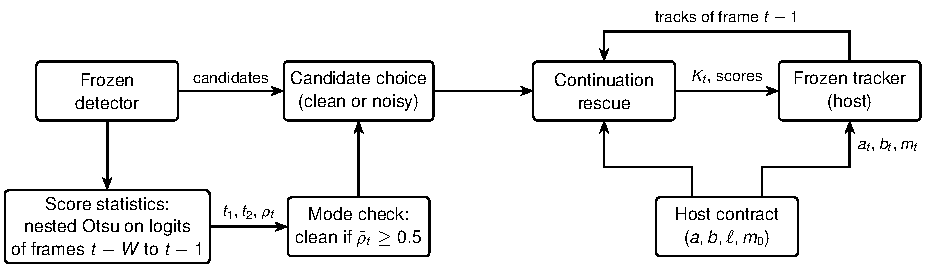
\includegraphics{Fig1.pdf}
\caption{\scl{} between a frozen detector and a frozen tracker (the host). Boxes are processing
steps and arrows show what each step passes on. The score statistics use earlier frames only. The
host contract holds the tracker's published settings. The tracker receives the chosen candidates
$K_t$, their scores, and its thresholds $a_t$, $b_t$ and tolerance $m_t$ for the frame}
\label{fig:arch}
\end{figure*}

\subsection{Inputs and outputs}\label{sec:problem}
In each frame $t$, the detector gives candidates $D_t=\{(\mathbf{x}_i,s_i,c_i)\}$, each with a box
$\mathbf{x}_i$, a score $s_i\in(0,1)$, and a class $c_i$. The layer works on the logit
\begin{equation}
z_i=\log\frac{s_i}{1-s_i},
\label{eq:logit}
\end{equation}
which spreads out scores close to 0 and 1; the logistic function $\sigma(z)=1/(1+e^{-z})$ turns it
back into a score. The host gives its contract $h=(a,b,\ell,m_0)$: the score $a$ needed to match a
track, the score $b$ needed to start one, the lowest score $\ell$ it uses, and its matching
tolerance $m_0$, one minus the smallest intersection over union (IoU) of two boxes that counts as a
match. A single-stage tracker has $\ell=\min(a,b)$, a two-stage tracker $\ell<\min(a,b)$. In
every frame the layer returns
\begin{equation}
\left(K_t,\tilde{s},a_t,b_t,m_t\right)=
\mathcal{L}\left(Z_{<t},D_t,\mathcal{T}_{t-1},g_t;\,h\right):
\label{eq:layer}
\end{equation}
the candidates $K_t$ for the tracker, their scores, and its thresholds and tolerance, from the
logits $Z_{<t}$ of earlier frames, the tracks $\mathcal{T}_{t-1}$, and a camera-motion measure
$g_t$; no future frame is used.

\subsection{Self-calibration from detector scores}\label{sec:calib}
The layer collects the logits $Z_t^W$ of the candidates of the last $W=10$ frames and splits them
twice with Otsu's method \cite{otsu1979}. The first split, $t_1$, separates background (low
logits) from foreground; the second, $t_2$, found on the foreground only, divides it into uncertain
and confident candidates. The share of confident candidates in the foreground,
\begin{equation}
\rho_t=\frac{\left|\{z\in Z_t^W: z\ge t_2\}\right|}{\left|\{z\in Z_t^W: z\ge t_1\}\right|},
\label{eq:rho}
\end{equation}
describes the shape of the score distribution and needs no labels: if 30 of 40 foreground
candidates are confident, $\rho_t=0.75$. Because the splits are made on logits, they move with the
scores when the whole logit scale is stretched or shifted, and each group keeps the same
candidates. Figure~\ref{fig:groups} shows the groups for a clean and a noisy stream. When a
detector emits very few low scores, the first split falls inside the objects; since clutter
usually gives more candidates than the objects do, a window with fewer candidates below $t_1$ than
above it counts as clean, $\rho_t=1$ (background check).

\begin{figure}[t]
\centering
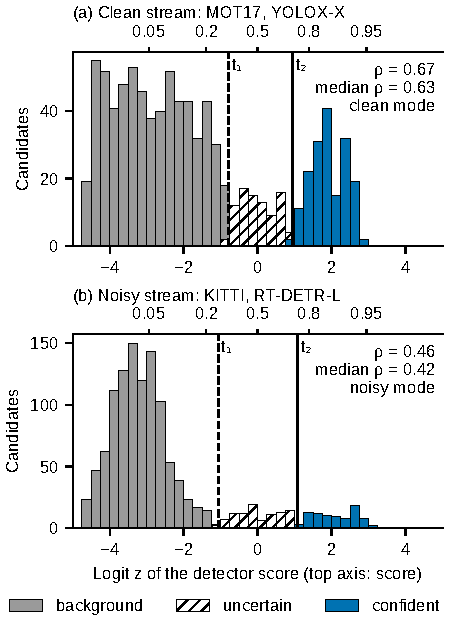
\includegraphics{Fig2.pdf}
\caption{What the layer sees: the logits of the candidates of the last 10 frames, just before its
decision for frame 101, with the Otsu splits $t_1$ (dashed line) and $t_2$ (solid line). Plain
light bars: background; hatched bars: uncertain; plain dark bars: confident. The top axis gives the
matching detector score. (a) MOT17-02 with YOLOX-X: most foreground candidates are confident, and
the stream is clean. (b) KITTI 0001 with RT-DETR-L: many are uncertain, and the stream is noisy.
Values of the frozen layer in the runs of Sect.~\ref{sec:results}}
\label{fig:groups}
\end{figure}

\subsection{Clean and noisy modes}\label{sec:regimes}
The stream is clean at frame $t$ if the median of all $\rho$ values so far is at least one half,
a majority rule, and noisy otherwise; before the first valid split it is cold. Because the median
covers the whole stream, a short drop in confidence does not change the mode, and during
development this whole-stream rule removed mode changes in the middle of streams that had lowered
HOTA (Sect.~\ref{sec:steps}). The splits themselves use only the last $W$ frames, so the groups, and
in the clean mode the threshold cap of Eq.~\eqref{eq:clean}, follow a change of the score scale
within $W$ frames even while the mode stays the same.

\emph{Cold and clean modes.} The tracker keeps its own thresholds and scores, and only cross-class
duplicates are removed. In the clean mode, a threshold so high that it would reject the confident
group is lowered to the score $\sigma(t_2)$ at which that group begins:
\begin{equation}
a_t=\min\!\left(a,\sigma(t_2)\right),\qquad b_t=\min\!\left(b,\sigma(t_2)\right).
\label{eq:clean}
\end{equation}
The clean mode is thus a minimal intervention rather than a plain pass-through: the scores are
kept, and the output equals that of the host alone whenever the confident group lies above the
host's thresholds and no rescue applies, as for BoostTrack, ByteTrack at floor 0.1, and Hybrid-SORT
on MOT17 (Sect.~\ref{sec:results}). When the scores are halved, for example, no score is above 0.5, and ByteTrack in
its official setting ($a=0.6$, $b=0.7$) never starts a track; the splits move with the halved
scores, so Eq.~\eqref{eq:clean} lets the confident candidates reach it again.

\emph{Noisy mode.} Confident candidates ($z\ge t_2$) may start and continue tracks, uncertain ones
($t_1\le z<t_2$) may only continue tracks, and background candidates are dropped. Each score is
replaced by its mid-rank $u_i\in(0,1)$ among the scores of a remap memory, which stores the scores
kept in the first frame and in every 10th frame, the last 20 of them (tied scores share their average
rank, and before the first sample the current frame is used),
\begin{equation}
\tilde{s}_i=
\begin{cases}
0.5+0.5\,u_i, & z_i\ge t_2,\\
0.1+0.4\,u_i, & t_1\le z_i<t_2,
\end{cases}
\label{eq:remap}
\end{equation}
and both thresholds are set to $a_t=b_t=0.5$, so uncertain candidates can only reach a tracker's
low-score step. A weaker candidate that overlaps a stronger one with IoU above one half is removed,
unless a different track of the previous frame claims it, which keeps people who stand close
together in a crowd.

\subsection{Track continuation and camera motion}\label{sec:rescue}
A track can be lost when its object gets low scores for a few frames, above all in single-stage
trackers, which have no low-score step. The rescue passes such a candidate, with its score raised
just above the lowest threshold of the frame, when it is in the foreground (or, for a
single-stage tracker, when there is no background group), overlaps a track of the previous frame
with IoU of at least one half, no other usable candidate covers that track, and the tracker could
not see it otherwise. It thus gives single-stage trackers the continuation step they lack.

In noisy frames, the matching tolerance also grows with camera motion. The motion is the shift
between consecutive grayscale frames at quarter resolution, found by phase correlation
\cite{reddy1996phasecorr}, and $r_t$ is its ratio to its median over the last 100 frames ($r_t=1$
during a warm-up of 5 frames or if this median is zero):
\begin{equation}
m_t=\min\!\left(0.95,\;1-\frac{1-m_0}{\max(1,r_t)}\right).
\label{eq:motion}
\end{equation}
With $m_0=0.8$ and twice the usual motion, a match needs an IoU of 0.1 instead of 0.2.

\subsection{Host contract and adapters}\label{sec:contract}
Table~\ref{tab:contracts} lists the contracts; each value is taken from the tracker's published
configuration, and none is fitted. For each tracker family, a small adapter writes the layer's
candidates, scores, thresholds, and tolerance into the tracker's existing parameters before each
update and then calls the tracker's own update. The matching steps, motion model, track
management, and any post-processing of the authors run unchanged, so the host stays frozen: its
code, weights, and association algorithm do not change, only the values of its thresholds are set
for each frame, and the rules are the same for every tracker.

\begin{table}[t]
\caption{Host contracts: the published settings of each tracker, as used by the layer: matching
(association) threshold $a$, birth threshold $b$, low threshold $\ell$, and match tolerance $m_0$.
For every tracker, the layer's decision is passed on as thresholds, candidates, and scores.}
\label{tab:contracts}
\centering\footnotesize
\setlength{\tabcolsep}{4pt}
\begin{tabular}{@{}>{\raggedright\arraybackslash}p{27mm}lcccc@{}}
\toprule
Tracker (setting) & Type & $a$ & $b$ & $\ell$ & $m_0$\\
\midrule
ByteTrack (official MOT17) & two-stage & 0.6 & 0.7 & 0.1 & 0.8\\
ByteTrack (library default) & two-stage & 0.25 & 0.25 & 0.1 & 0.8\\
BoT-SORT (library default) & two-stage & 0.25 & 0.25 & 0.1 & 0.8\\
SparseTrack & two-stage & 0.6 & 0.7 & 0.1 & 0.85\\
BoostTrack & two-stage & 0.6 & 0.6 & 0.1 & 0.7\\
Hybrid-SORT & two-stage & 0.6 & 0.6 & 0.1 & 0.75\\
OC-SORT & single-stage & 0.6 & 0.6 & 0.6 & 0.7\\
PD-SORT & single-stage & 0.6 & 0.6 & 0.6 & 0.7\\
\bottomrule
\end{tabular}
\end{table}


\subsection{Parameter values}\label{sec:constants}
Table~\ref{tab:constants} lists all values of \scl{}. They were fixed before the external
evaluation, are the same for every tracker, detector, and dataset, and none was chosen by searching
over a range of values. They come from standard values (the IoU of 0.5 of MOT evaluation and the
common thresholds 0.5 and 0.1), from definitions, and from design choices kept fixed in all
development stages.

\begin{table}[t]
\caption{Values of \scl{} and their source.}
\label{tab:constants}
\centering\footnotesize
\setlength{\tabcolsep}{3pt}
\begin{tabular}{@{}>{\raggedright\arraybackslash}p{19mm}>{\raggedright\arraybackslash}p{27mm}>{\raggedright\arraybackslash}p{25mm}@{}}
\toprule
Value & Setting & Source\\
\midrule
Window $W$ & 10 frames & design choice\\
Mode rule & clean if median $\rho\ge0.5$ & majority rule\\
Background check & $\rho=1$ if fewer below $t_1$ than above & rule: no background group\\
Noisy score ranges & $[0.5,1)$, $[0.1,0.5)$ & common thresholds\\
Noisy $a_t$, $b_t$ & 0.5 & common threshold\\
Remap memory & 20 frames, one every 10 & design choice\\
Duplicate, rescue IoU & 0.5 & MOT evaluation IoU\\
Rescued score & lowest threshold $+\,0.001$ & just above the threshold\\
Motion cue & phase correlation, quarter resolution & standard method \cite{reddy1996phasecorr}\\
Motion history & 100 frames, warm-up 5 & design choice\\
Tolerance cap & 0.95 & minimum overlap 0.05\\
\bottomrule
\end{tabular}
\end{table}

\subsection{Per-frame steps and cost}\label{sec:cost}
Algorithm~\ref{alg:layer} gives the steps for one frame. With $n$ candidates and $k$ tracks, the
cost is $O(Wn\log(Wn)+n^2+nk)$, for sorting the window and comparing candidates with each other and
with the tracks, plus one phase correlation on a small image; the whole-stream mode stores one
$\rho$ value per frame and takes their median. Table~\ref{tab:runtime} gives the
measured time per frame of a full pipeline on an ordinary processor.

\begin{table}[t]
\caption{Baseline comparison of the per-frame time on a 4-vCPU Intel Xeon
(2.10 GHz, no GPU) with a live YOLOv8n detector (736 pixels) and ByteTrack on
three KITTI sequences (2,279 timed frames per arm). Host alone: the same
pipeline without \scl{}. Mean / 95th percentile in milliseconds.}
\label{tab:runtime}
\centering\footnotesize
\setlength{\tabcolsep}{4pt}
\begin{tabular}{@{}lcc@{}}
\toprule
Stage & Host alone & Host + \scl{}\\
\midrule
Frame decode & 13.88 / 16.21 & 13.88 / 16.51\\
Detector (YOLOv8n, 736 px) & 41.91 / 58.41 & 42.17 / 59.43\\
\scl{} & -- & 2.95 / 4.39\\
Tracker (ByteTrack) & 2.04 / 3.57 & 1.43 / 2.64\\
End to end & 57.85 / 76.35 & 60.44 / 80.78\\
\bottomrule
\end{tabular}
\end{table}


\begin{algorithm}[t]
\caption{\scl{} for frame $t$. The window holds the logits of frames
$t-W$ to $t-1$, so the decision for frame $t$ uses no future frame.}\label{alg:layer}
\begin{algorithmic}[1]
\Require candidates $D_t$, tracks $\mathcal{T}_{t-1}$, motion cue $g_t$, contract $(a,b,\ell,m_0)$, constants of Table~\ref{tab:constants}
\Ensure candidates $K_t$, scores $\tilde{s}$, thresholds $a_t,b_t$, tolerance $m_t$
\State $z_i\gets$ logit of $s_i$ for all $i$ \Comment{Eq.~\eqref{eq:logit}}
\If{no valid split exists} \Comment{e.g., first frame}
  \State mode $\gets$ cold; $(a_t,b_t)\gets(a,b)$
\Else
  \State $(t_1,t_2)\gets$ nested Otsu on the window \Comment{Sect.~\ref{sec:calib}}
  \State $\rho_t\gets$ Eq.~\eqref{eq:rho} with the background check
  \State mode $\gets$ clean if $\mathrm{median}(\rho)\ge0.5$, else noisy
\EndIf
\If{mode is cold or clean} \Comment{Sect.~\ref{sec:regimes}}
  \State remove cross-class duplicates; keep raw scores
  \If{clean} set $(a_t,b_t)$ by Eq.~\eqref{eq:clean}
  \EndIf
\Else \Comment{noisy mode}
  \State remove duplicates with track context
  \State drop $z<t_1$; remap scores by Eq.~\eqref{eq:remap}
  \State $a_t\gets0.5$; $b_t\gets0.5$
\EndIf
\State rescue continuations (not cold) \Comment{Sect.~\ref{sec:rescue}}
\State $m_t\gets$ Eq.~\eqref{eq:motion} if noisy, else $m_0$
\State pass $K_t$, $\tilde{s}$, $a_t$, $b_t$, $m_t$ to the tracker
\State add the logits left after duplicate removal to the window
\State add $g_t$ to the motion history
\State store the tracks of frame $t$ after the tracker update
\end{algorithmic}
\end{algorithm}

\section{Development of the Final SCL}\label{sec:development}

\scl{} was developed in three stages on the development data of Sect.~\ref{sec:data}: a starting
point, design steps that each removed one cause found before them, and a freeze before any external
test.

\subsection{Starting point: always-on banding}\label{sec:prior}
The earlier design \aob{} computed the same nested Otsu groups but treated every stream as noisy:
in every frame it applied the groups, removed every weaker candidate that overlapped a stronger one
with IoU above one half, and rescored all candidates by rank. Table~\ref{tab:prior} compares \aob{}
and \scl{} with strong published trackers on MOT17. \aob{} lowered the HOTA of SparseTrack by 4.15
points and of BoostTrack by 5.89 points online and 5.37 points with its gap-filling post-processing
(GBI), for two reasons: removing overlapping boxes deleted people hidden behind others in crowds,
and its thresholds were stricter than the trackers' own. With the same trackers, \scl{} changed
HOTA by $+0.06$ for SparseTrack and left both BoostTrack versions identical to the host. A layer
that acts in every frame therefore cannot be placed safely in front of an unknown tracker, and the
next steps let the layer decide from the scores whether to act at all.

\begin{table}[t]
\caption{Baseline comparison of the development stage on MOT17 val-half
(published YOLOX-X detections). Host: the tracker alone, without any
layer (our run of the published tracker). $\Delta$: tracker with the earlier design \aob{} or with \scl{}
minus host, with 95\% paired-bootstrap interval (10,000 resamples,
seed 42). Bold intervals exclude zero. IDS: identity switches, a count
(lower is better).}
\label{tab:prior}
\centering\footnotesize
\setlength{\tabcolsep}{3pt}
\renewcommand{\arraystretch}{1.1}
\begin{tabular}{@{}lrcc@{}}
\toprule
Metric & Host & $\Delta$ \aob{} & $\Delta$ \scl{}\\
\midrule
\multicolumn{4}{@{}l}{\textit{SparseTrack} \cite{liu2025sparsetrack}}\\
\quad HOTA & 68.88 & \cibt{-4.15}{-5.54}{-1.66} & \cit{+0.06}{-0.01}{+0.25}\\
\quad MOTA & 77.85 & \cibt{-6.14}{-8.10}{-2.74} & \cit{+0.08}{-0.03}{+0.30}\\
\quad IDF1 & 81.97 & \cibt{-4.49}{-6.19}{-1.96} & \cit{+0.16}{-0.02}{+0.70}\\
\quad IDS & 124 & \cit{-16}{-47}{+12} & \cit{+7}{0}{+19}\\
\multicolumn{4}{@{}l}{\textit{BoostTrack, online} \cite{stanojevic2024boosttrack}}\\
\quad HOTA & 68.49 & \cibt{-5.89}{-7.76}{-2.87} & 0 (identical)\\
\quad MOTA & 75.50 & \cibt{-8.87}{-12.37}{-7.14} & 0 (identical)\\
\quad IDF1 & 81.41 & \cibt{-6.22}{-9.33}{-2.85} & 0 (identical)\\
\quad IDS & 113 & \cibt{-38}{-81}{-1} & 0 (identical)\\
\multicolumn{4}{@{}l}{\textit{BoostTrack, with GBI} \cite{stanojevic2024boosttrack}}\\
\quad HOTA & 71.72 & \cibt{-5.37}{-7.30}{-2.75} & 0 (identical)\\
\quad MOTA & 81.03 & \cibt{-8.73}{-12.59}{-6.50} & 0 (identical)\\
\quad IDF1 & 84.16 & \cibt{-5.65}{-8.96}{-2.77} & 0 (identical)\\
\quad IDS & 97 & \cit{-27}{-73}{+11} & 0 (identical)\\
\bottomrule
\end{tabular}
\end{table}


\subsection{Design steps}\label{sec:steps}
Each step was compared with the step before it (Table~\ref{tab:ablation}). The \emph{mode gate}
added the mode check, the clean mode that keeps the tracker's scores and thresholds, and the crowd-safe duplicate
rule; it restored SparseTrack from 64.72 to 68.93 HOTA and BoostTrack from 62.61 to 68.37. The
\emph{whole-stream mode} removed mode changes in the middle of streams and raised ByteTrack from
67.561 to 67.702 and OC-SORT from 65.697 to 66.071. The \emph{continuation rescue} added 0.2 to 0.4
points for OC-SORT. The \emph{background check} completed \scl{}: ByteTrack and BoostTrack returned
to output identical to the host, and OC-SORT rose to 67.04 and 66.91 at the two floors. Four other
variants were tested and not kept.

\begin{table*}[tp]
\caption{Design steps from \aob{} to \scl{} on development
data (HOTA, \%), and versions that were tested and rejected. The floor of
ByteTrack and OC-SORT is given in parentheses.}
\label{tab:ablation}
\centering\footnotesize
\setlength{\tabcolsep}{4pt}
\begin{tabular}{@{}>{\raggedright\arraybackslash}p{25mm}>{\raggedright\arraybackslash}p{36mm}>{\raggedright\arraybackslash}p{62mm}@{}}
\toprule
Step & Change & Effect\\
\midrule
\aob{} emulated & always-noisy bands, overlap deduplication, rank remap & ByteTrack (0.1) 56.41 vs host 67.70; OC-SORT (0.1) 45.72 vs 66.44\\
+ mode gate & mode statistic, host-anchored clean mode, crowd-safe duplicates & SparseTrack 64.72 to 68.93 (host 68.88); BoostTrack 62.61 to 68.37 (host 68.49)\\
+ whole-stream mode & mode from all past frames & ByteTrack (0.1) 67.561 to 67.702; OC-SORT (0.1) 65.697 to 66.071\\
+ continuation rescue & foreground track-consistent rescue & OC-SORT (0.01) 66.405 to 66.619; OC-SORT (0.1) 66.071 to 66.469\\
+ background check = \scl{} & no background mode gives no evidence against the host & ByteTrack/BoostTrack (0.1) identical to host; OC-SORT 67.041 (0.01), 66.907 (0.1)\\
\midrule
\multicolumn{2}{@{}l}{\textit{Rejected version}} & \textit{Evidence}\\
\multicolumn{2}{@{}l}{no candidates at frame 1} & $-0.3$ to $-0.5$ HOTA on every MOT17 host\\
\multicolumn{2}{@{}l}{rescue below a two-stage host's low stage} & FP $+700$ to $+1000$, $-0.4$ to $-0.5$ HOTA\\
\multicolumn{2}{@{}l}{rank-remapped scores in clean frames} & ByteTrack $-0.2$ / $-1.6$ HOTA\\
\multicolumn{2}{@{}l}{host-clipped noisy primary band} & KITTI YOLOv8n ByteTrack $+1.4$ HOTA but uncontrolled false tracks on a noisy aerial stream (26.9 vs 14.9 boxes/frame)\\
\bottomrule
\end{tabular}
\end{table*}


\subsection{Freezing and testing}\label{sec:freeze}
The final configuration was frozen before any external test as a version-control tag, protected
by a lock file with a cryptographic hash of the layer, its configuration, and the evaluation
scripts. Sixty-one automated tests check, among others, that the layer uses no future data and
passes clean streams unchanged.

\section{Results}\label{sec:results}

A tracker that fits its detector should keep its accuracy, and one that does not, because it lacks
a continuation step or because the detector or its scores changed, should gain. For each host, the
baseline is the host alone (Host in the tables), run with its published configuration and the same
detections; the second run adds the frozen \scl{} and changes nothing else. Figure~\ref{fig:forest} summarizes the HOTA difference for every tested cell.

\begin{figure}[t]
\centering
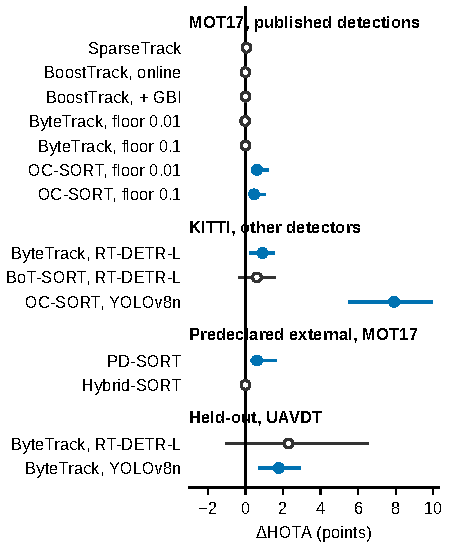
\includegraphics{Fig3.pdf}
\caption{Difference in HOTA, host with \scl{} minus host alone, in points, for every tested cell,
with its 95\% paired-bootstrap interval. Filled circles: interval above zero; open circles:
interval contains zero, or identical output}
\label{fig:forest}
\end{figure}

\subsection{MOT17 evaluation across trackers}\label{sec:tracker}
Table~\ref{tab:mot17} shows the development trackers on MOT17 val-half. The two-stage trackers with
well-matched detections stayed at the accuracy of their hosts: BoostTrack, online and with GBI, and
ByteTrack at floor 0.1 gave exactly the same output, and ByteTrack at floor 0.01 and SparseTrack
stayed within 0.06 HOTA points, the self-limiting clean mode. The single-stage OC-SORT improved at
both floors (HOTA $+0.61$ and $+0.46$, MOTA $+1.27$ and $+1.26$), with fewer identity switches and
higher HOTA on 7 of 7 sequences, through the continuation rescue.

\begin{table}[tp]
\caption{Baseline comparison of the development trackers on MOT17 val-half
(published YOLOX-X detections). Paper: number reported by the tracker's
authors. Host: the tracker alone, without \scl{} (our run of the published tracker). $\Delta$: host with
\scl{} minus host, with 95\% paired-bootstrap interval (10,000
resamples, seed 42); bold intervals exclude zero. The floor is the lowest
detector score emitted. IDS: identity switches, a count (lower is better);
--: not reported by the authors.}
\label{tab:mot17}
\centering\footnotesize
\setlength{\tabcolsep}{4pt}
\begin{tabular}{@{}lrrl@{}}
\toprule
Metric & Paper & Host & $\Delta$ [95\% CI]\\
\midrule
\multicolumn{4}{@{}l}{\textit{SparseTrack} \cite{liu2025sparsetrack}}\\
\quad HOTA & 69.2 & 68.88 & $+0.06$ [$-0.01$, $+0.25$]\\
\quad MOTA & 76.8 & 77.85 & $+0.08$ [$-0.03$, $+0.30$]\\
\quad IDF1 & 81.4 & 81.97 & $+0.16$ [$-0.02$, $+0.70$]\\
\quad IDS & -- & 124 & $+7$ [$0$, $+19$]\\
\multicolumn{4}{@{}l}{\textit{BoostTrack, online} \cite{stanojevic2024boosttrack}}\\
\quad HOTA & 68.37 & 68.49 & 0 (identical)\\
\quad MOTA & 75.56 & 75.50 & 0 (identical)\\
\quad IDF1 & 81.35 & 81.41 & 0 (identical)\\
\quad IDS & 118 & 113 & 0 (identical)\\
\multicolumn{4}{@{}l}{\textit{BoostTrack, + GBI} \cite{stanojevic2024boosttrack}}\\
\quad HOTA & 71.33 & 71.72 & 0 (identical)\\
\quad MOTA & 80.55 & 81.03 & 0 (identical)\\
\quad IDF1 & 83.84 & 84.16 & 0 (identical)\\
\quad IDS & 106 & 97 & 0 (identical)\\
\multicolumn{4}{@{}l}{\textit{ByteTrack, floor 0.01} \cite{zhang2022bytetrack}}\\
\quad HOTA & -- & 67.70 & $-0.014$ [$-0.058$, $+0.009$]\\
\quad MOTA & 76.6 & 77.60 & $+0.06$ [$-0.15$, $+0.34$]\\
\quad IDF1 & 79.3 & 79.47 & $-0.031$ [$-0.135$, $+0.035$]\\
\quad IDS & -- & 214 & $+4$ [$-2$, $+13$]\\
\multicolumn{4}{@{}l}{\textit{ByteTrack, floor 0.1} \cite{zhang2022bytetrack}}\\
\quad HOTA & -- & 67.70 & 0 (identical)\\
\quad MOTA & 76.6 & 77.60 & 0 (identical)\\
\quad IDF1 & 79.3 & 79.47 & 0 (identical)\\
\quad IDS & -- & 214 & 0 (identical)\\
\multicolumn{4}{@{}l}{\textit{OC-SORT, floor 0.01} \cite{cao2023ocsort}}\\
\quad HOTA & 66.5 & 66.43 & {\boldmath $+0.61$ [$+0.36$, $+1.24$]}\\
\quad MOTA & 74.9 & 74.67 & {\boldmath $+1.27$ [$+0.17$, $+3.01$]}\\
\quad IDF1 & 77.7 & 78.05 & $+0.66$ [$-0.25$, $+1.60$]\\
\quad IDS & -- & 211 & {\boldmath $-8$ [$-15$, $-2$]}\\
\multicolumn{4}{@{}l}{\textit{OC-SORT, floor 0.1} \cite{cao2023ocsort}}\\
\quad HOTA & 66.5 & 66.44 & {\boldmath $+0.46$ [$+0.27$, $+1.09$]}\\
\quad MOTA & 74.9 & 74.67 & {\boldmath $+1.26$ [$+0.37$, $+3.34$]}\\
\quad IDF1 & 77.7 & 78.05 & {\boldmath $+0.287$ [$+0.003$, $+0.838$]}\\
\quad IDS & -- & 213 & $-14$ [$-38$, $+6$]\\
\bottomrule
\end{tabular}
\end{table}


\subsection{KITTI evaluation with other detectors}\label{sec:detector}
Table~\ref{tab:kitti} shows what happens when the detector is replaced. With the noisy RT-DETR-L,
ByteTrack gained 5.98 MOTA, 3.87 IDF1, and 0.91 HOTA points, and BoT-SORT 7.86 MOTA and 3.10 IDF1
points, with 297 and 226 fewer identity switches. With YOLOv8n, OC-SORT gained 7.91 HOTA
points ($[+5.47,+9.98]$), 9.40 MOTA points, and 9.60 IDF1 points; it followed many more objects, as
its missed objects (FN) fell by 5,310, and its identity switches rose with them by 79.
Figure~\ref{fig:example} follows this cell over three frames: each object keeps its ID,
and at frame 102 OC-SORT alone tracked 6 of the 10 labelled objects and with \scl{} 9.

\begin{table}[tp]
\caption{Baseline comparison under a detector change on KITTI tracking
training (official HOTA, car and pedestrian averaged). Host: the tracker
alone, without \scl{}, with the same detections. $\Delta$: host with \scl{}
minus host, with 95\% paired-bootstrap interval; bold intervals exclude zero.
IDS: identity switches, a count (lower is better). BoT-SORT: KITTI sequence 0020
is left out of both runs, because the BoT-SORT code stopped with a numerical
error in its Kalman update on it; the other 20 sequences are used.}
\label{tab:kitti}
\centering\footnotesize
\setlength{\tabcolsep}{4pt}
\begin{tabular}{@{}lrl@{}}
\toprule
Metric & Host & $\Delta$ [95\% CI]\\
\midrule
\multicolumn{3}{@{}l}{\textit{ByteTrack} \cite{zhang2022bytetrack}\textit{, RT-DETR-L}}\\
\quad HOTA & 50.73 & {\boldmath $+0.91$ [$+0.22$, $+1.55$]}\\
\quad MOTA & 47.27 & {\boldmath $+5.98$ [$+1.16$, $+9.94$]}\\
\quad IDF1 & 64.98 & {\boldmath $+3.87$ [$+1.67$, $+5.06$]}\\
\quad IDS & 686 & {\boldmath $-297$ [$-530$, $-122$]}\\
\multicolumn{3}{@{}l}{\textit{BoT-SORT} \cite{aharon2022botsort}\textit{, RT-DETR-L} (20 sequences)}\\
\quad HOTA & 53.91 & $+0.61$ [$-0.39$, $+1.61$]\\
\quad MOTA & 48.25 & {\boldmath $+7.86$ [$+2.21$, $+13.44$]}\\
\quad IDF1 & 67.74 & {\boldmath $+3.10$ [$+1.00$, $+4.57$]}\\
\quad IDS & 476 & {\boldmath $-226$ [$-369$, $-120$]}\\
\multicolumn{3}{@{}l}{\textit{OC-SORT} \cite{cao2023ocsort}\textit{, YOLOv8n}}\\
\quad HOTA & 36.27 & {\boldmath $+7.91$ [$+5.47$, $+9.98$]}\\
\quad MOTA & 33.99 & {\boldmath $+9.40$ [$+1.10$, $+12.30$]}\\
\quad IDF1 & 50.46 & {\boldmath $+9.60$ [$+5.61$, $+12.16$]}\\
\quad IDS & 91 & {\boldmath $+79$ [$+43$, $+125$]}\\
\bottomrule
\end{tabular}
\end{table}


\begin{figure*}[t]
\centering
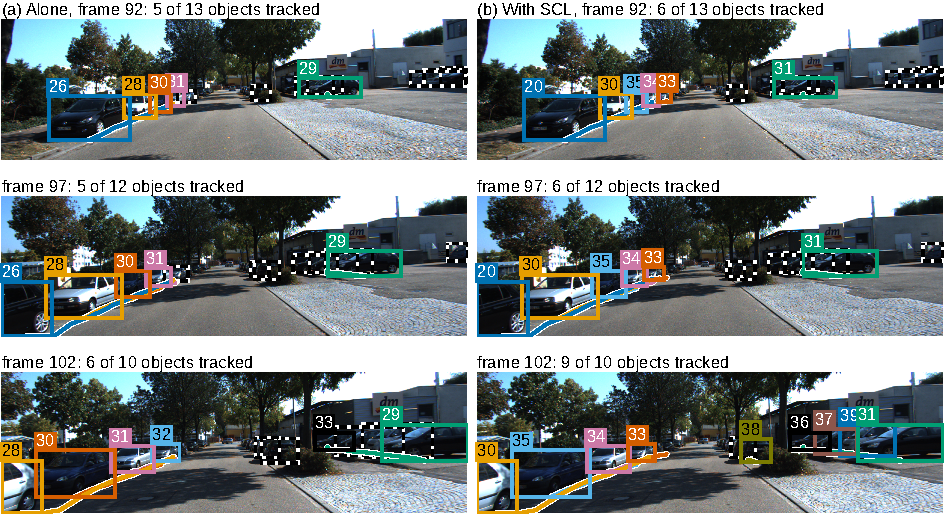
\includegraphics{Fig4.pdf}
\caption{Tracking on KITTI sequence 0001 \cite{geiger2012kitti} with OC-SORT and YOLOv8n, at
frames 92, 97, and 102 (rows): (a) the tracker alone, (b) with \scl{}. Each output track keeps one
ID and one colour over the frames; the line of the same colour is its path over the previous 20
frames (bottom centre of its box). Dashed boxes: labelled objects that no track covers. IDs are
numbered separately in each run. The sequence has the median HOTA gain of the 21 sequences, and
frame 102 is its first frame with the largest gain in tracked objects}
\label{fig:example}
\end{figure*}

\subsection{Evaluation under shifted detector scores}\label{sec:shift}
Table~\ref{tab:shift} shows the trackers under the four score transforms. Halving the scores
reduced ByteTrack (official setting) and OC-SORT to 0 HOTA; with the layer they reached 66.17 and
66.72. Cubing reduced them to 60.92 and 58.34, and the layer restored them to 65.81 and 66.60;
BoostTrack rose from 61.33 to 64.84. With $T=2$, the layer raised ByteTrack and OC-SORT by 1.11 and
1.24 points. The library setting of ByteTrack, whose low thresholds already accept the changed
scores, stayed within 0.14 points. Over the 14 conditions, the layer raised HOTA significantly in 7
and lowered it significantly in none.

\begin{table}[tp]
\caption{Baseline comparison under shifted detector scores on MOT17 val-half. The detector
scores are transformed before the tracker, whose published thresholds stay fixed; $T$ is a logit
temperature, $\sigma(z/T)$. Host: the tracker alone, without \scl{}. $\Delta$: with \scl{} minus host,
with 95\% paired-bootstrap interval (10,000 resamples, seed 42); bold intervals exclude zero.
Emission floor 0.01 (BoostTrack 0.1).}
\label{tab:shift}
\centering\footnotesize
\setlength{\tabcolsep}{4pt}
\begin{tabular}{@{}lrrl@{}}
\toprule
 & \multicolumn{3}{c}{HOTA (\%)}\\
\cmidrule(l){2-4}
Transform & Host & + \scl{} & $\Delta$ [95\% CI]\\
\midrule
\multicolumn{4}{@{}l}{\textit{ByteTrack, official setting} \cite{zhang2022bytetrack}}\\
\quad $s^3$ & 60.92 & 65.81 & {\boldmath $+4.89$ [$+2.60$, $+13.69$]}\\
\quad $0.5\,s$ & 0.00 & 66.17 & {\boldmath $+66.17$ [$+49.32$, $+75.40$]}\\
\quad $T=2$ & 65.84 & 66.95 & {\boldmath $+1.11$ [$+0.35$, $+3.87$]}\\
\quad $T=0.5$ & 67.30 & 67.29 & $-0.009$ [$-0.051$, $+0.005$]\\
\multicolumn{4}{@{}l}{\textit{ByteTrack, library setting} \cite{zhang2022bytetrack}}\\
\quad $s^3$ & 66.31 & 66.31 & $-0.006$ [$-0.384$, $+0.383$]\\
\quad $0.5\,s$ & 66.61 & 66.48 & $-0.14$ [$-0.66$, $+0.14$]\\
\quad $T=2$ & 63.97 & 63.97 & 0 (identical)\\
\quad $T=0.5$ & 66.53 & 66.52 & $-0.006$ [$-0.029$, $+0.001$]\\
\multicolumn{4}{@{}l}{\textit{OC-SORT} \cite{cao2023ocsort}}\\
\quad $s^3$ & 58.34 & 66.60 & {\boldmath $+8.26$ [$+5.86$, $+16.81$]}\\
\quad $0.5\,s$ & 0.00 & 66.72 & {\boldmath $+66.72$ [$+50.32$, $+75.56$]}\\
\quad $T=2$ & 65.99 & 67.22 & {\boldmath $+1.24$ [$+0.52$, $+3.42$]}\\
\quad $T=0.5$ & 66.61 & 67.06 & $+0.45$ [$-0.01$, $+0.97$]\\
\multicolumn{4}{@{}l}{\textit{BoostTrack, online} \cite{stanojevic2024boosttrack}}\\
\quad $s^3$ & 61.33 & 64.84 & {\boldmath $+3.51$ [$+0.85$, $+13.28$]}\\
\quad $T=2$ & 67.59 & 67.59 & 0 (identical)\\
\bottomrule
\end{tabular}
\end{table}


\subsection{Comparison with adaptive-threshold methods}\label{sec:baselines}
\begin{table}[tp]
\caption{HOTA (\%) of \scl{} and of two simple adaptive-threshold baselines on KITTI tracking
training (official HOTA, car and pedestrian averaged). Host: the tracker alone, without any layer.
$t_1$, $t_2$: the adaptive baselines, in which the tracker's matching and birth thresholds are set in every frame to the
first or second Otsu split of the logits of the last 10 frames, and the scores are passed unchanged.
Halved: halved detector scores. $\Delta$: \scl{} minus the $t_2$ baseline, with 95\% paired-bootstrap interval below the
value; bold intervals exclude zero.}
\label{tab:baselines}
\centering\footnotesize
\setlength{\tabcolsep}{3pt}
\begin{tabular}{@{}lrrrrc@{}}
\toprule
Cell & Host & $t_1$ & $t_2$ & \scl{} & $\Delta$\\
\midrule
\twol{OC-SORT,}{YOLOv8n} & 36.27 & 39.97 & 41.09 & 44.17 & \cib{+3.09}{+2.00}{+4.03}\\
\addlinespace[3pt]
\begin{tabular}[c]{@{}l@{}}ByteTrack,\\RT-DETR-L,\\halved\end{tabular} & 49.50 & 49.58 & 49.50 & 51.78 & \cib{+2.29}{+0.28}{+4.96}\\
\addlinespace[3pt]
\begin{tabular}[c]{@{}l@{}}OC-SORT,\\YOLOv8n,\\halved\end{tabular} & 0.00 & 37.68 & 43.56 & 46.30 & \cib{+2.74}{+1.32}{+3.34}\\
\bottomrule
\end{tabular}
\end{table}

\begin{table*}[tp]
\caption{HOTA of ACT \cite{act2026adaptive} and of \scl{} on the same detections, and the
differences \scl{} minus ACT in HOTA and IDF1, with 95\% paired-bootstrap interval below each
value; bold intervals exclude zero. ACT: published parameters, no
tuning. KITTI: official HOTA, car and pedestrian averaged; MOT17: val-half, ACT's own setting;
UAVDT: test split, one vehicle class, ignored regions removed (Sect.~\ref{sec:metrics}).}
\label{tab:act}
\centering\footnotesize
\setlength{\tabcolsep}{5pt}
\begin{tabular}{@{}lllrrcc@{}}
\toprule
Data & Detector & Tracker & ACT & \scl{} & $\Delta$HOTA & $\Delta$IDF1\\
\midrule
KITTI, halved scores & RT-DETR-L & ByteTrack & 49.77 & 51.78 & \cib{+2.01}{+0.01}{+4.76} & \ci{+1.70}{-1.13}{+6.80}\\
KITTI, halved scores & YOLOv8n & OC-SORT & 36.24 & 46.30 & \cib{+10.06}{+6.88}{+12.01} & \cib{+12.03}{+6.85}{+14.69}\\
\addlinespace[4pt]
MOT17, floor 0.01 & YOLOX-X & ByteTrack (official) & 67.46 & 67.68 & \ci{+0.22}{-0.43}{+0.88} & \ci{+0.57}{-0.68}{+2.12}\\
MOT17, floor 0.1 & YOLOX-X & ByteTrack (official) & 67.46 & 67.70 & \ci{+0.23}{-0.40}{+0.90} & \ci{+0.60}{-0.55}{+2.10}\\
\addlinespace[4pt]
UAVDT test & YOLOv8n & ByteTrack & 29.01 & 30.83 & \cib{+1.82}{+0.65}{+3.00} & \cib{+4.00}{+1.85}{+6.22}\\
UAVDT test & RT-DETR-L & ByteTrack & 40.14 & 42.37 & \ci{+2.23}{-0.97}{+6.32} & \ci{+5.35}{-0.03}{+12.47}\\
\bottomrule
\end{tabular}
\end{table*}

Two simple baselines set the tracker's matching and birth thresholds in every frame to the first or
second Otsu split of the logits of the last 10 frames, $t_1$ or $t_2$, and pass the scores
unchanged. On KITTI (Table~\ref{tab:baselines}), \scl{} reached the highest HOTA in all three
cells, 2.2 to 8.6 points above the baselines, with intervals against the $t_2$ baseline above zero
in every cell, so adaptive thresholds alone do not explain the gains. With OC-SORT, \scl{} also had
fewer identity switches than both baselines (170 against 1,545 and 250 with YOLOv8n; 308 against
1,975 and 492 under halved scores).

ACT \cite{act2026adaptive} was run with its published parameters, without retuning, on the same detections
(Table~\ref{tab:act}). \scl{} reached higher HOTA than ACT in every row, significantly under halved
scores ($+2.01$ and $+10.06$ points) and with YOLOv8n on UAVDT ($+1.82$), and also in the MOT17
setting for which ACT was designed. With RT-DETR-L on UAVDT, \scl{} reached a MOTA of 27.99 against
5.34 ($+22.65$, $[+9.03,+47.21]$), because the fixed score levels of ACT removed few of the host's
false positives (178,219 against 78,975). \scl{} also had fewer identity switches than ACT on
MOT17 and UAVDT (up to 418 fewer).

Removing one part at a time on KITTI shows where the gains come from: without the rescue, HOTA
fell by up to 3.35 points; without the mode decision, by up to 2.44; and without the new scores of
the noisy mode, by up to 1.67.


\subsection{Frozen evaluation on external trackers}\label{sec:external}
\begin{table}[tp]
\caption{Baseline comparison on the predeclared external systems (MOT17
val-half, authors' released detections), each evaluated once with the frozen
\scl{}. Paper: number reported by the authors (for PD-SORT, their released
output). Host: the tracker alone, without \scl{} (our run of the published tracker). Reproduction class
against the authors' number (EXACT: $|\Delta\mathrm{HOTA}|\le0.2$; CLOSE:
$\le1.0$ with a documented, untuned cause). $\Delta$: host with \scl{} minus
host, with 95\% paired-bootstrap interval; bold intervals exclude zero. IDS:
identity switches, a count (lower is better); --: not reported.}
\label{tab:external}
\centering\footnotesize
\setlength{\tabcolsep}{4pt}
\begin{tabular}{@{}lrrl@{}}
\toprule
Metric & Paper & Host & $\Delta$ [95\% CI]\\
\midrule
\multicolumn{4}{@{}l}{\textit{PD-SORT} \cite{wang2025pdsort}\textit{, EXACT}}\\
\quad HOTA & 68.01 & 68.01 & {\boldmath $+0.61$ [$+0.27$, $+1.65$]}\\
\quad MOTA & 75.19 & 75.19 & {\boldmath $+1.13$ [$+0.27$, $+3.03$]}\\
\quad IDF1 & 81.03 & 81.03 & {\boldmath $+0.82$ [$+0.43$, $+1.94$]}\\
\quad IDS & -- & 129 & $+2$ [$-9$, $+13$]\\
\multicolumn{4}{@{}l}{\textit{Hybrid-SORT} \cite{yang2024hybridsort}\textit{, CLOSE}}\\
\quad HOTA & 67.1 & 66.70 & 0 (identical)\\
\quad MOTA & 75.8 & 75.52 & 0 (identical)\\
\quad IDF1 & 78.0 & 77.56 & 0 (identical)\\
\quad IDS & -- & 259 & 0 (identical)\\
\bottomrule
\end{tabular}
\end{table}

Table~\ref{tab:external} gives the two predeclared external systems. PD-SORT \cite{wang2025pdsort}
was reproduced exactly. With \scl{}, its HOTA rose by 0.61 points ($[+0.27,+1.65]$), its MOTA by
1.13 ($[+0.27,+3.03]$), and its IDF1 by 0.82 ($[+0.43,+1.94]$), with higher HOTA on 7 of 7
sequences; like OC-SORT, it is a single-stage tracker, but it was not seen during design.
Hybrid-SORT \cite{yang2024hybridsort}, a two-stage tracker, gave identical output, as predicted
before the run.


\subsection{Frozen UAVDT transfer}\label{sec:visdrone}
\begin{table}[tp]
\caption{Baseline comparison on the held-out UAVDT test split (20 aerial
sequences, not used during design), evaluated once with the frozen \scl{}. Host: ByteTrack alone, without \scl{}, with its published setting. $\Delta$: host
with \scl{} minus host, with 95\% paired-bootstrap interval; bold intervals
exclude zero. IDS: identity switches, a count (lower is better).}
\label{tab:visdrone}
\centering\footnotesize
\setlength{\tabcolsep}{4pt}
\begin{tabular}{@{}lrl@{}}
\toprule
Metric & Host & $\Delta$ [95\% CI]\\
\midrule
\multicolumn{3}{@{}l}{\textit{ByteTrack, RT-DETR-L} \cite{zhang2022bytetrack,zhao2024rtdetr}}\\
\quad HOTA & 40.07 & $+2.30$ [$-1.05$, $+6.55$]\\
\quad MOTA & 3.29 & {\boldmath $+24.70$ [$+10.06$, $+51.08$]}\\
\quad IDF1 & 48.59 & {\boldmath $+5.74$ [$+0.13$, $+13.11$]}\\
\quad IDS & 1041 & {\boldmath $-586$ [$-951$, $-248$]}\\
\multicolumn{3}{@{}l}{\textit{ByteTrack, YOLOv8n} \cite{zhang2022bytetrack,jocher2023yolov8}}\\
\quad HOTA & 29.05 & {\boldmath $+1.77$ [$+0.70$, $+2.94$]}\\
\quad MOTA & 16.27 & $+1.02$ [$-1.06$, $+2.86$]\\
\quad IDF1 & 34.52 & {\boldmath $+3.97$ [$+1.88$, $+6.17$]}\\
\quad IDS & 719 & {\boldmath $-326$ [$-691$, $-73$]}\\
\bottomrule
\end{tabular}
\end{table}

On the held-out UAVDT test split (Table~\ref{tab:visdrone}), \scl{} raised the HOTA of the YOLOv8n
stream by 1.77 points ($[+0.70,+2.94]$) and its IDF1 by 3.97 points, and cut identity switches by
45\%. With RT-DETR-L, whose host produced many false positives (MOTA 3.29), \scl{} raised MOTA by
24.70 points ($[+10.06,+51.08]$) and IDF1 by 5.74 points, and cut false positives by 58\% and
identity switches by 56\%. No HOTA decrease was detected with either detector.


\section{Discussion}\label{sec:discussion}

\emph{The score scale is part of the MOT system.} Halving the scores reduced ByteTrack and OC-SORT
from 67.70 and 66.43 HOTA to 0, and with RT-DETR-L on UAVDT ByteTrack reached a MOTA of only 3.29.
The fixed thresholds of a tracker hold only for the detector they were tuned for, so the score
scale deserves the same attention as the association method.

\emph{Self-limiting by design.} In the clean mode the layer keeps the tracker's thresholds and
scores, so a well-matched tracker receives its normal input; \aob{}, which always intervened,
lowered the same trackers by 4.15 to 5.89 HOTA points. Single-stage trackers gain through the
rescue, and two-stage trackers when the detector is noisy.

\emph{Deployment.} \scl{} needs no training, no GPU, and no access to the inside of the detector or
the tracker. On a CPU it takes 2.95 ms per frame, small next to the 42 ms of the detector, and the
tracker itself ran faster with it (1.43 against 2.04 ms per frame); the end-to-end time rose by
only 4.5\% (Table~\ref{tab:runtime}). A new tracker is added through its four published contract
values and an adapter, without changes to the rules.

\section{Conclusion}\label{sec:conclusion}

This paper presented \scl{}, a training-free layer between an unchanged detector and an unchanged
tracker. Nested Otsu splits of recent logits decide whether the scores are clean or noisy; on clean
scores the layer keeps the tracker's scores and, where they fit, its thresholds, on noisy scores it chooses the candidates, rescores
them, and sets the thresholds, and a continuation rescue gives single-stage trackers the step they
lack. One frozen configuration restored two trackers from 0 to about 66 HOTA under halved scores,
improved both single-stage trackers on every MOT17 sequence, raised MOTA by up to 24.70 points on
held-out aerial data, reached higher HOTA than simple adaptive thresholds and ACT, kept well-matched
trackers at their own accuracy with no statistically detected HOTA loss, and took 2.95 ms per frame on a CPU. The score scale of the detector should therefore be treated as part of
the tracking system. Future work will test the layer with more detectors, trackers, and datasets.


\backmatter

\bibliography{references}

\end{document}
